\chapter{Embedded Programming}
The learning objectes of this chapter are embedded systems in general, and the Arduino case study.

Embedded systems are systems that are designed to perform a specific task, and they are usually part of a larger system.
Hardware and software are often designed together, aka ``hardware-software co-design''.
They are typically based on microcontrollers, optimized for controlling I/O.
They are often used in \ul{\textbf{real-time} systems, where timing is crucial}.

Many types of microcontrollers are availble on the market:
\begin{itemize}
   \item ``General purpose'', meaning that can be adapted to several embedded applications
   \item ``Application specific integrated circuit''(\texttt{ASIC}s) which are very efficient and performative, but tightly bound to a specific task
   \item ``System on a chip''(\texttt{SoC}s) which are a combination of a microcontroller and other components, like a radio module. 
   \note{The term is very broad, and it can refer to a wide range of devices.}
\end{itemize}

When programming on microcontrollers it must be taken into account the \textbf{small memory footprint}, the absence of user interfaces, file systems, OSs.
In general is not possible to program and compile code directly, or to control the program execution with a user interface.

\framedt{Programming Challenges}{
   \begin{itemize}
      \item Timing correctness
      \item High reliability 
      \item Often impossible to use debuggers
      \item Efficient use of memory
      \item Power management
   \end{itemize}
}

\section{Executable and SW organization}
When a device starts it executes the \texttt{main} program, which first initializes device peripherals and then enters an infinite loop, implementing the functionalities of the device.
Such loop naturally defines a duty cycle, typically consisting of:
\begin{itemize}
   \item Reading from transducers
   \item Taking a decision
   \item Controlling actuators
   \item Optionally communicating with other devices
\end{itemize}

At low-level, the code interacts with the device hardware by means of commands and interrupts. In conventional OSs insteads commands are available in terms of system calls, which are later handled by the OS.

\section{Different Models to implement duty cycles}
\subsection{Arduino Model}
\begin{figure}[htbp]
   \centering
   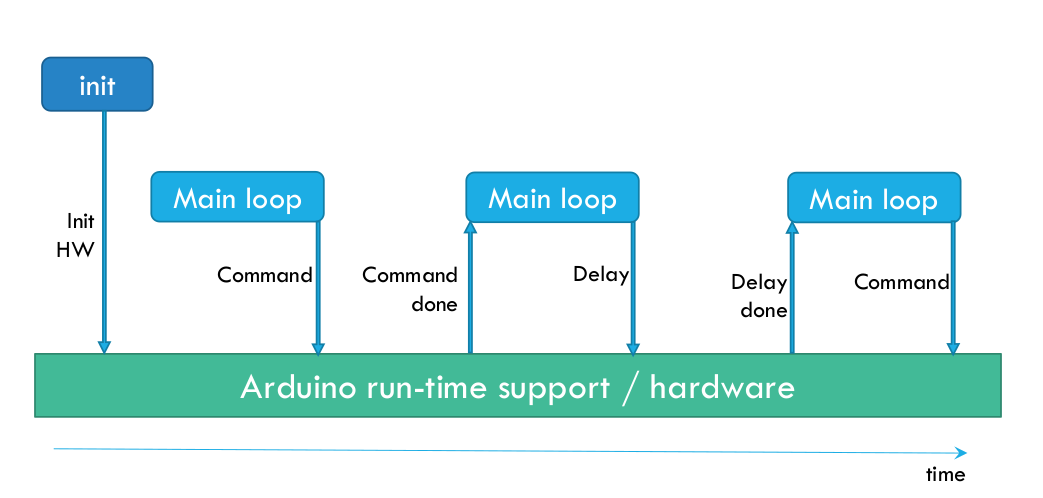
\includegraphics{images/arduino_model.png}
   \caption{Sample flow of execution in Arduino.}
   \label{fig:arduino_model}
\end{figure}
The job of Arduino is defined in a single loop function, which clearly may invoke other functions anyway.
Such loop is executed repeatedly by a \ul{\textit{single} thread which is \textit{never} suspended}.
In case of an I/O operation, the program waits for the operation to complete, and then continues.

\subsection{TinyOS Model}

TinyOS offers functions (\textbf{commands}) to program and activate the hardware, it abstracts interrupts in form of \textit{events}.
It defines non-preemptive tasks that are executed sequentially, to manage different activities.

With this approach a task never waits. However interrupts should be handled as soon
as they arrive by means of an event handler, which should be as short as possible; tasks can be pre-empted (only) by events.

\begin{figure}[htbp]
   \centering
   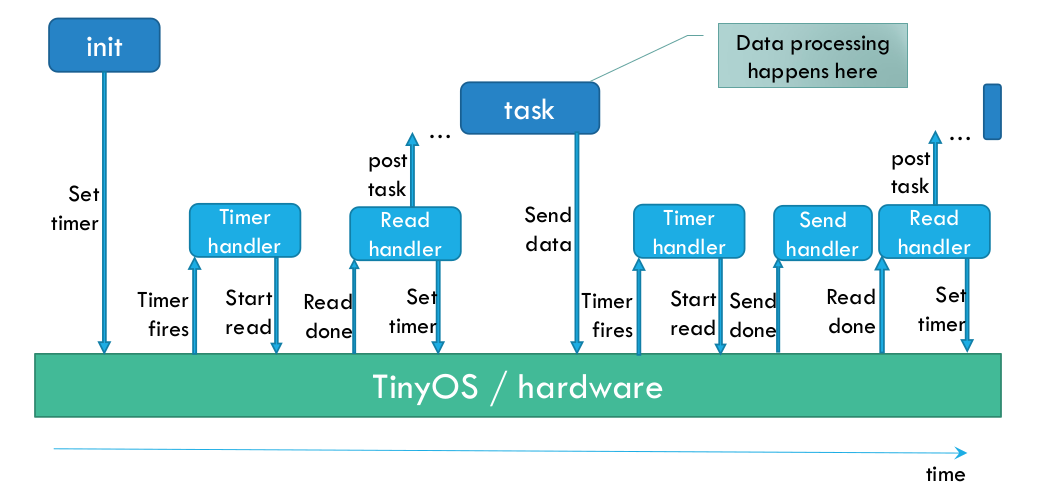
\includegraphics{images/tinyos_model.png}
   \caption{Sample flow of execution in TinyOS.}
   \label{fig:tinyos_model}
\end{figure}

\section{Arduino}

TODO \dots

\subsection{Interrupts}
There are three types of interrupts in Arduino:
\begin{itemize}
   \item \textbf{External}:
   a signal outside Arduino coming from a pin
   \item \textbf{Timer}:
   internal Arduino timer 
   \item \textbf{Device}:
   internal signal coming from a device such as ADC, serial line, etc.
\end{itemize}

Internal interrupts (either Timer or Device) are managed by
the run time support of Arduino, external ones instead may be managed with an \lstinline|attachInterrupt(interrupt#, func-name,mode);| instruction.


\subsection{Question on the slides}
\begin{lstlisting}
   void setup(){
      pinMode(2, INPUT);
      attachInterrupt(0, handler, CHANGE);
      return;
   }
   
   void handler(){}
   
   void loop(){
      return;
   }
\end{lstlisting}